% standalone source of Fig. 1 (pdflatex figures/overview.tex); the Access class clashes with TikZ, so the
% manuscript includes the compiled PDF.  Keep the algorithm numbers in sync with main.tex.
\documentclass[border=2pt]{standalone}
\usepackage{amsmath}
\usepackage{tikz}
\usetikzlibrary{positioning,arrows.meta,fit,shapes.misc}
\begin{document}
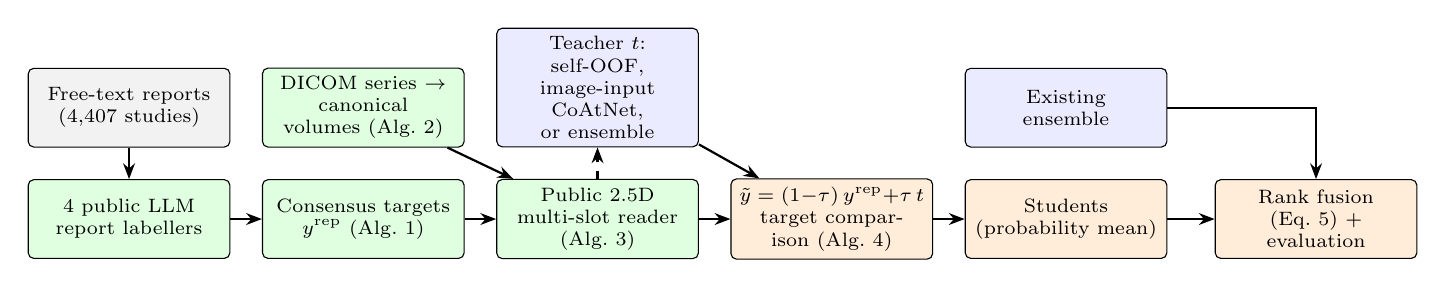
\begin{tikzpicture}[
  node distance=4mm and 4mm,
  box/.style={draw, rounded corners=2pt, align=center, font=\scriptsize, minimum height=10mm, inner sep=3pt, fill=white, text width=2.35cm},
  data/.style={box, fill=gray!10},
  ours/.style={box, fill=orange!15},
  ext/.style={box, fill=blue!8},
  reused/.style={box, fill=green!12},
  arr/.style={-{Stealth[length=2mm]}, thick}]
\node[data] (rep) {Free-text reports\\(4,407 studies)};
\node[reused, below=of rep] (llm) {4 public LLM\\report labellers};
\node[reused, right=of llm] (v0) {Consensus targets\\$y^{\mathrm{rep}}$ (Alg.~1)};
\node[reused, above=of v0] (dcm) {DICOM series $\rightarrow$\\canonical\\volumes (Alg.~2)};
\node[reused, right=of v0] (rd) {Public 2.5D\\multi-slot reader\\(Alg.~3)};
\node[ext, above=of rd] (teach) {Teacher $t$: self-OOF,\\image-input CoAtNet,\\or ensemble};
\node[ours, right=of rd] (mix) {$\tilde{y}=(1-\tau)\,y^{\mathrm{rep}}+\tau\,t$\\target comparison (Alg.~4)};
\node[ours, right=of mix] (stu) {Students\\(probability mean)};
\node[ext, above=of stu] (par) {Existing\\ensemble};
\node[ours, right=of stu, xshift=2mm] (fin) {Rank fusion\\(Eq.~5) + evaluation};
\draw[arr] (rep) -- (llm);
\draw[arr] (llm) -- (v0);
\draw[arr] (v0) -- (rd);
\draw[arr] (dcm) -- (rd);
\draw[arr] (rd) -- (mix);
\draw[arr] (teach) -- (mix);
\draw[arr] (mix) -- (stu);
\draw[arr] (stu) -- (fin);
\draw[arr] (par) -| (fin);
\draw[arr, dashed] (rd) -- (teach);
\end{tikzpicture}
\end{document}
